\section{Fit test}
\label{app:FitTest}

\subsection{Data fit with $t\Bar{t}+\text{light}$ constrained}
\label{subapp:DataFit_w_ttlight_constrained}

\subsubsection{Pre-fit plots}
This section tests data fits with $t\Bar{t}+\text{light}$ constrained to the result of $t\Bar{t}$ cross-section measurement using boosted top-quarks in $\ell+\text{jets}$ channel \cite{aad2022measurements}. The analysis obtained the fiducial cross-sections of $\sigma_{\text{data}} = 1.267 \pm 0.005 \pm 0.053$ and $\sigma_{\text{MC}} = 1.481 + 0.091 - 0.083$ from collision data and $t\Bar{t}$ MC (PP8), respectively. From these results, the normalization of $t\Bar{t}$ MC (PP8) is expected to be as follows:
\begin{equation}
    \frac{\sigma_{\text{data}}}{\sigma_{\text{MC}}} \sim 0.856 + 0.074 - 0.070
\end{equation}

We perform fitting to data (BOnly) with $t\Bar{t}+\text{light}$ fixed after scaling by 0.856. The uncertainties of $\pm 1\sigma$ are introduced as an NP.  Figure \ref{fig:Prefit_Hp1000_Blind_with_ttlight_constrained} to \ref{fig:Prefit_Hp5000_Blind_with_ttlight_constrained} show the pre-fit plots for each $H^{+}$ mass hypothesis. 

\begin{figure}[H]
  \centering
  \subfloat[]{
    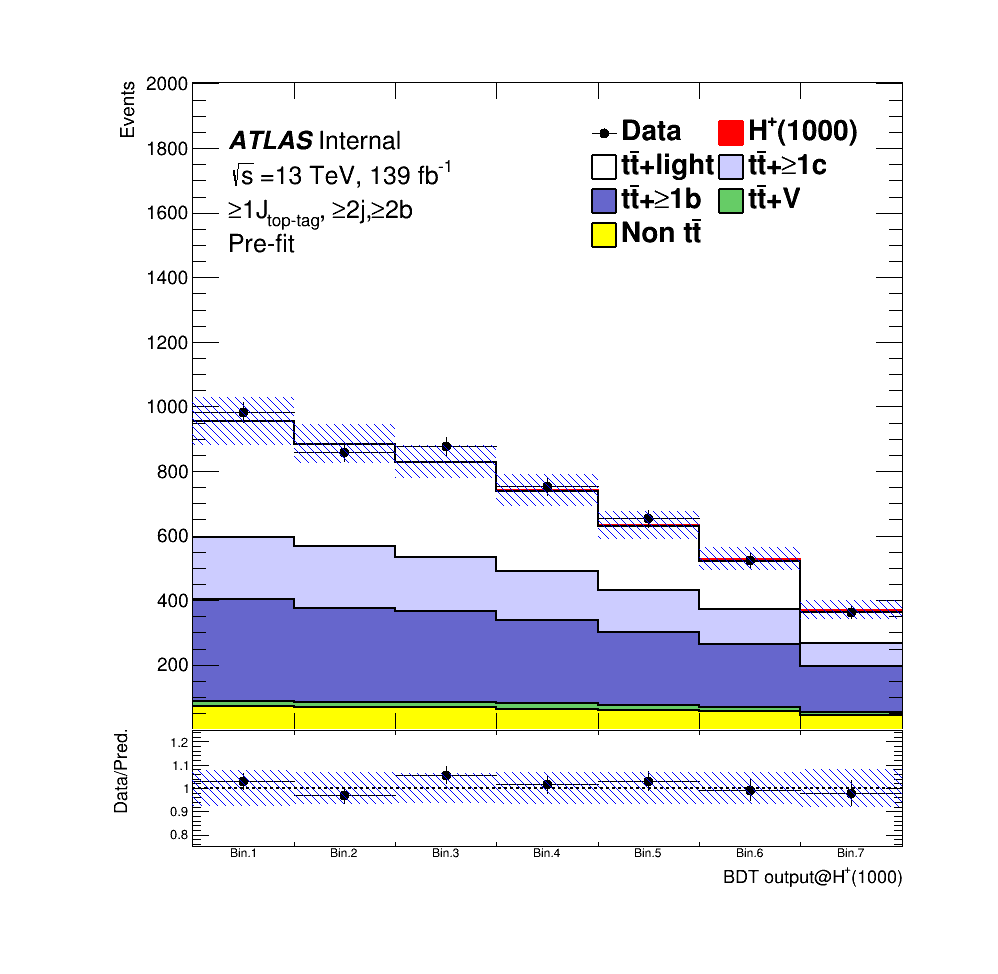
\includegraphics[width=0.45\textwidth]{images/FitTest/Prefit_Hp1000_blind_w_ttl_scaled_SR.png}
  }
  \subfloat[]{
    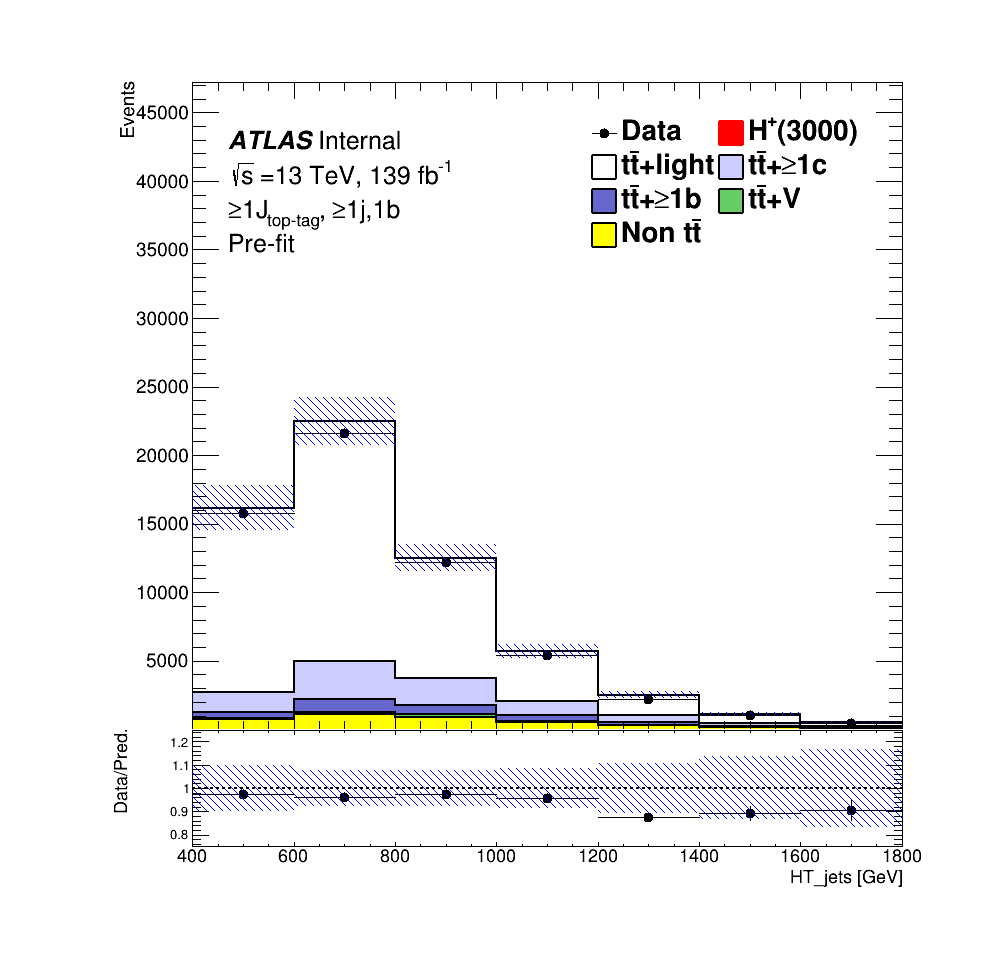
\includegraphics[width=0.45\textwidth]{images/FitTest/Prefit_Hp1000_blind_w_ttl_scaled_CR.png}
  }
  \caption{Pre-fit plots in the SR (left) and CR (right) for 1000 GeV mass hypothesis of $H^{+}$ signal. The blinded bins aren't plotted. $t\Bar{t}+\text{light}$ MC events are scaled by 0.856. The uncertainties of $+0.074$ and $-0.070$ are included as systematics. The scale factor and uncertainties are the ratio of fiducial cross-sections of collision data and $t\Bar{t}$ MC (PP8), which are obtained by $t\Bar{t}$ cross-section measurement analysis using boosted top-quarks in $\ell+\text{jets}$ channel.}
  \label{fig:Prefit_Hp1000_Blind_with_ttlight_constrained}
\end{figure}
\begin{figure}[H]
  \centering
  \subfloat[]{
    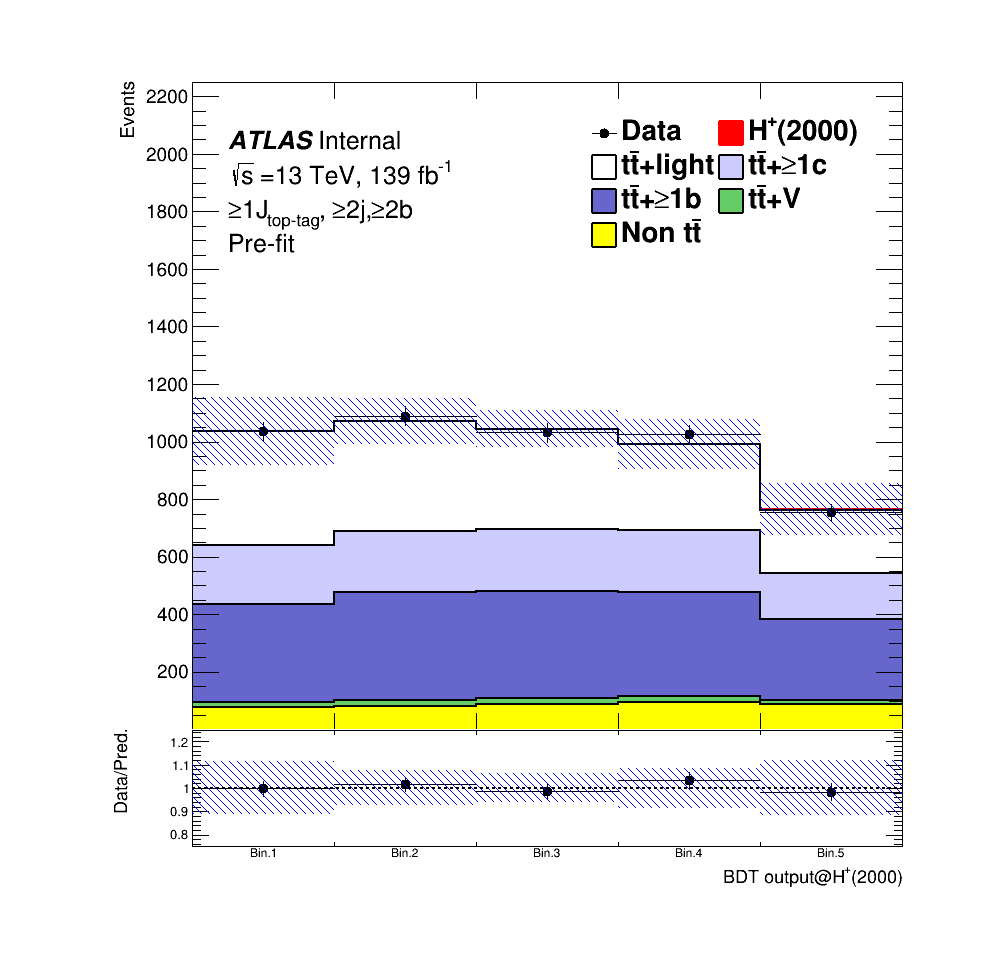
\includegraphics[width=0.45\textwidth]{images/FitTest/Prefit_Hp2000_blind_w_ttl_scaled_SR.png}
  }
  \subfloat[]{
    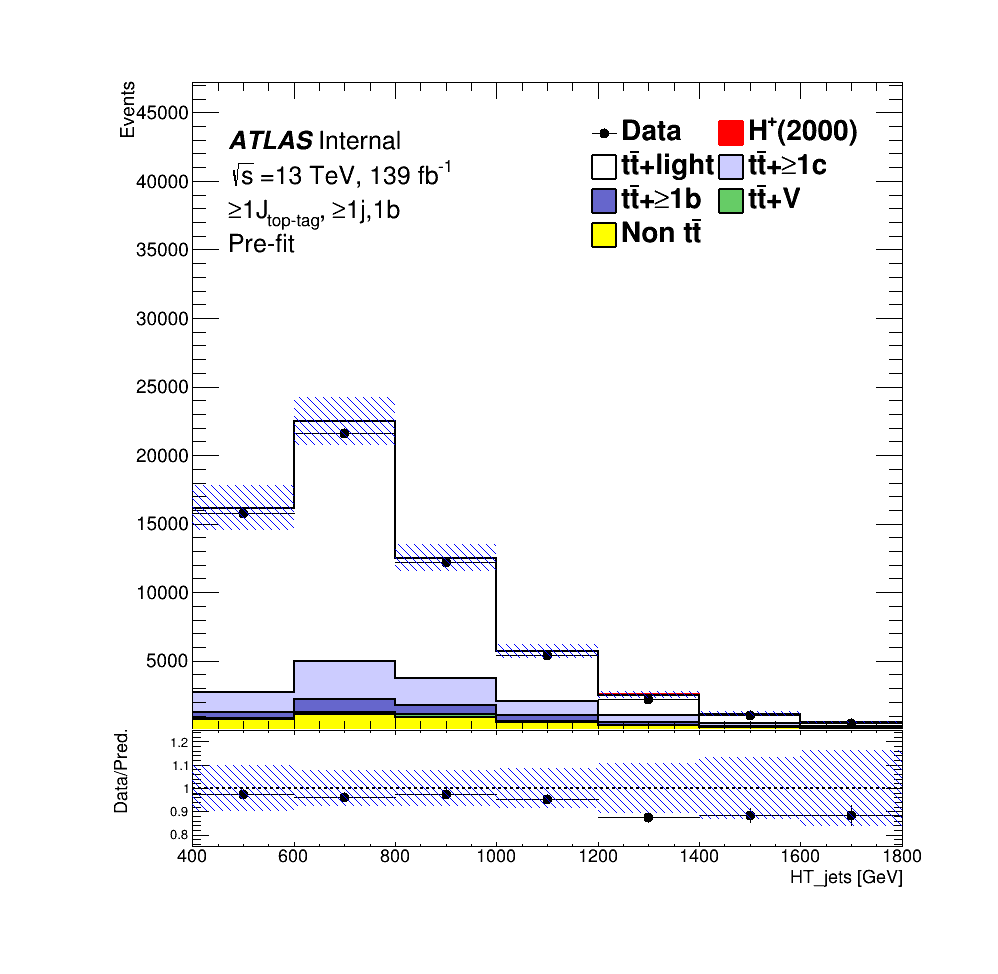
\includegraphics[width=0.45\textwidth]{images/FitTest/Prefit_Hp2000_blind_w_ttl_scaled_CR.png}
  }
  \caption{Pre-fit plots in the SR (left) and CR (right) for 2000 GeV mass hypothesis of $H^{+}$ signal. The blinded bins aren't plotted. $t\Bar{t}+\text{light}$ MC events are scaled by 0.856. The uncertainties of $+0.074$ and $-0.070$ are included as systematics. The scale factor and uncertainties are the ratio of fiducial cross-sections of collision data and $t\Bar{t}$ MC (PP8), which are obtained by $t\Bar{t}$ cross-section measurement analysis using boosted top-quarks in $\ell+\text{jets}$ channel.}
  \label{fig:Prefit_Hp2000_Blind_with_ttlight_constrained}
\end{figure}
\begin{figure}[H]
  \centering
  \subfloat[]{
    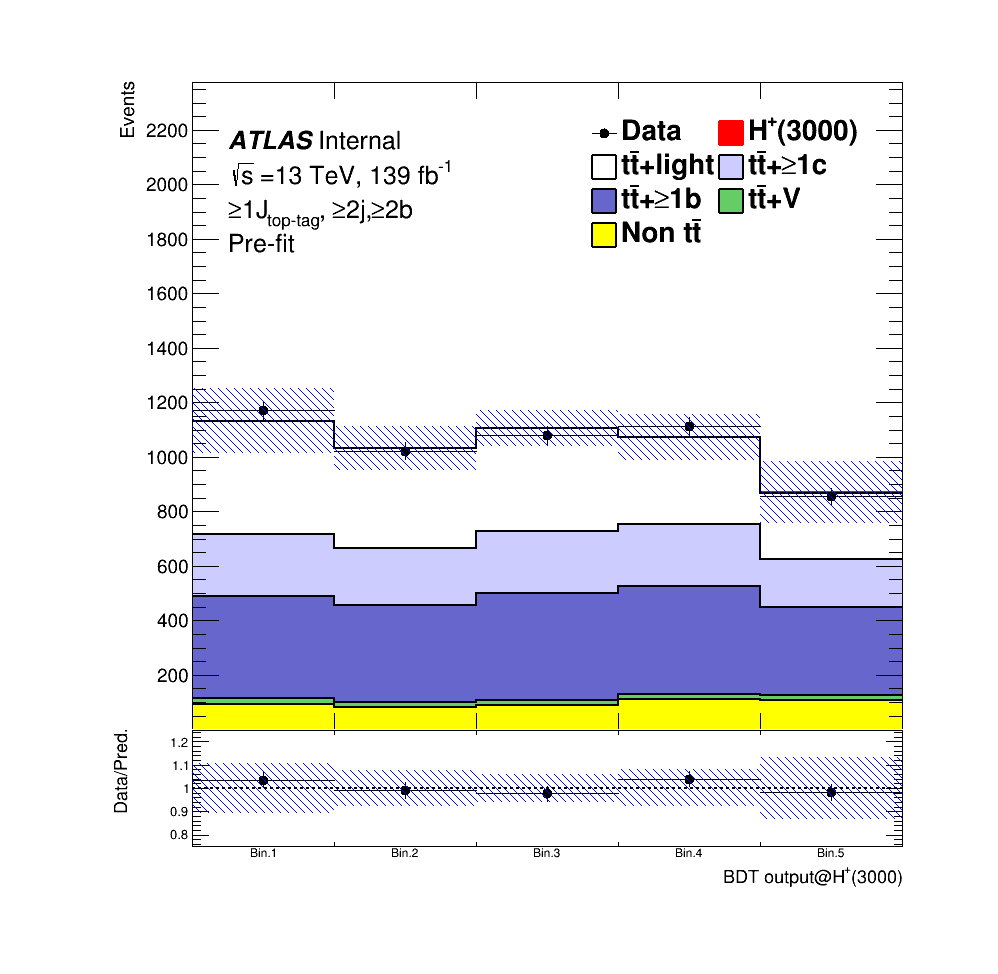
\includegraphics[width=0.45\textwidth]{images/FitTest/Prefit_Hp3000_blind_w_ttl_scaled_SR.png}
  }
  \subfloat[]{
    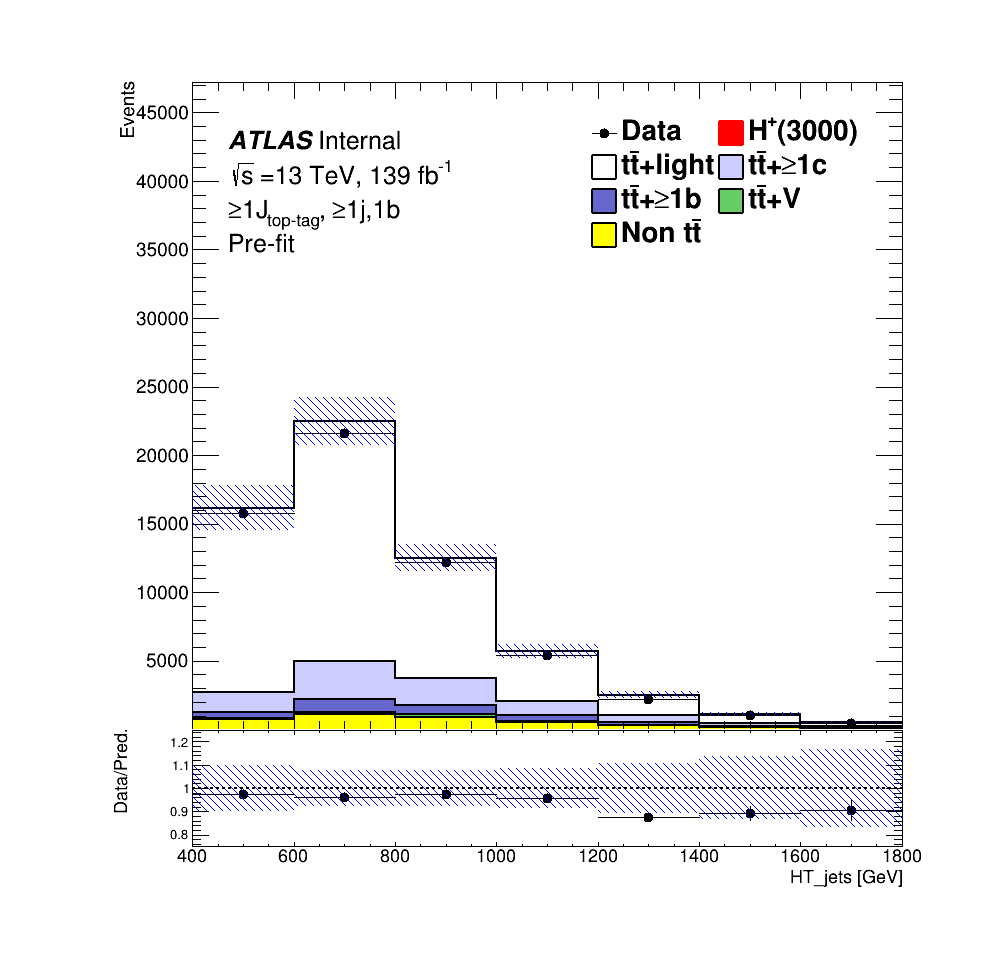
\includegraphics[width=0.45\textwidth]{images/FitTest/Prefit_Hp3000_blind_w_ttl_scaled_CR.png}
  }
  \caption{Pre-fit plots in the SR (left) and CR (right) for 3000 GeV mass hypothesis of $H^{+}$ signal. The blinded bins aren't plotted. $t\Bar{t}+\text{light}$ MC events are scaled by 0.856. The uncertainties of $+0.074$ and $-0.070$ are included as systematics. The scale factor and uncertainties are the ratio of fiducial cross-sections of collision data and $t\Bar{t}$ MC (PP8), which are obtained by $t\Bar{t}$ cross-section measurement analysis using boosted top-quarks in $\ell+\text{jets}$ channel.}
  \label{fig:Prefit_Hp3000_Blind_with_ttlight_constrained}
\end{figure}
\begin{figure}[H]
  \centering
  \subfloat[]{
    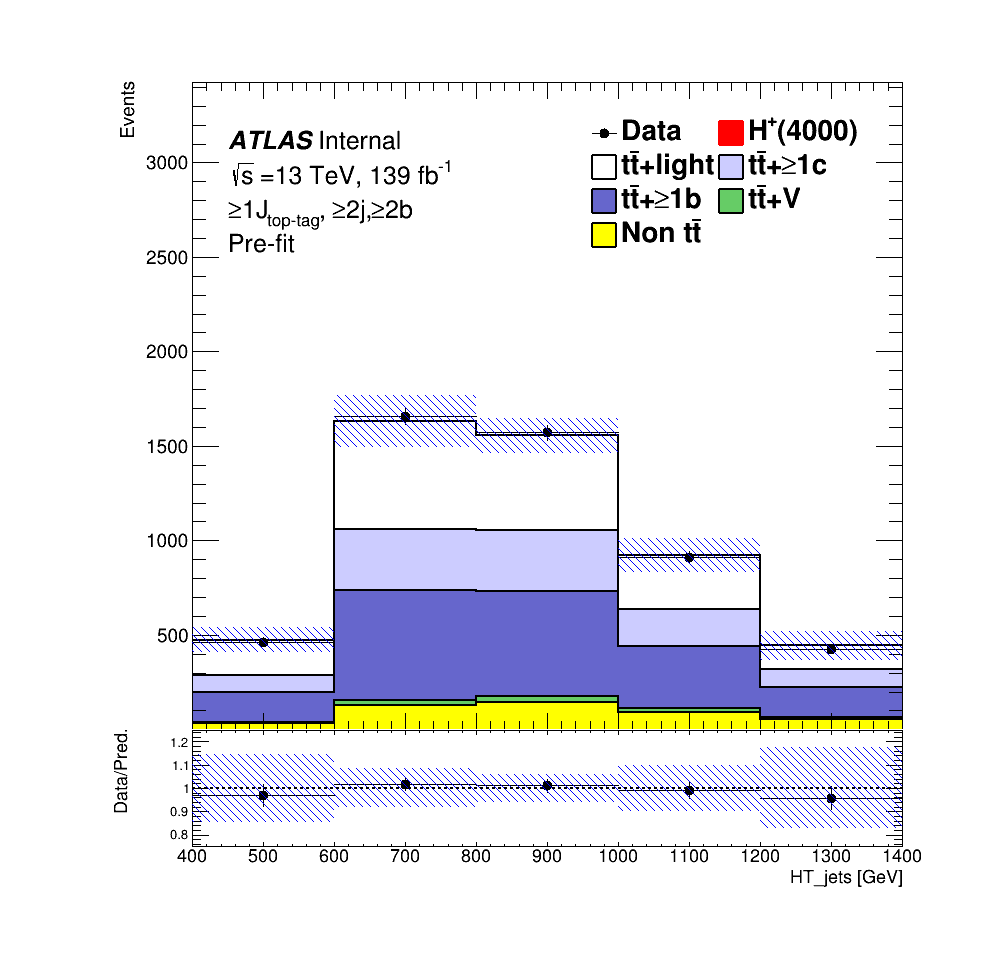
\includegraphics[width=0.45\textwidth]{images/FitTest/Prefit_Hp4000_blind_w_ttl_scaled_CR1.png}
  }
  \subfloat[]{
    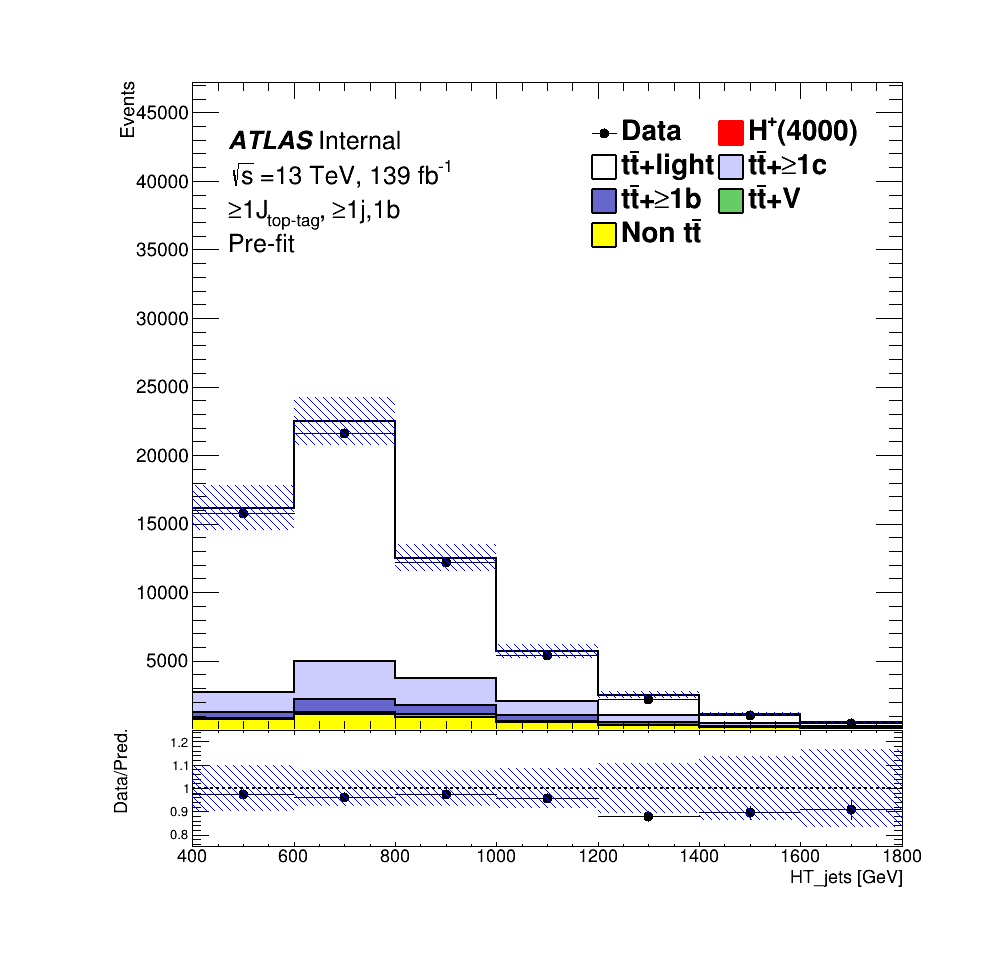
\includegraphics[width=0.45\textwidth]{images/FitTest/Prefit_Hp4000_blind_w_ttl_scaled_CR2.png}
  }
  \caption{Pre-fit plots in the CR1 (left) and CR2 (right) for 4000 GeV mass hypothesis of $H^{+}$ signal. The blinded bins aren't plotted. $t\Bar{t}+\text{light}$ MC events are scaled by 0.856. The uncertainties of $+0.074$ and $-0.070$ are included as systematics. The scale factor and uncertainties are the ratio of fiducial cross-sections of collision data and $t\Bar{t}$ MC (PP8), which are obtained by $t\Bar{t}$ cross-section measurement analysis using boosted top-quarks in $\ell+\text{jets}$ channel.}
  \label{fig:Prefit_Hp4000_Blind_with_ttlight_constrained}
\end{figure}
\begin{figure}[H]
  \centering
  \subfloat[]{
    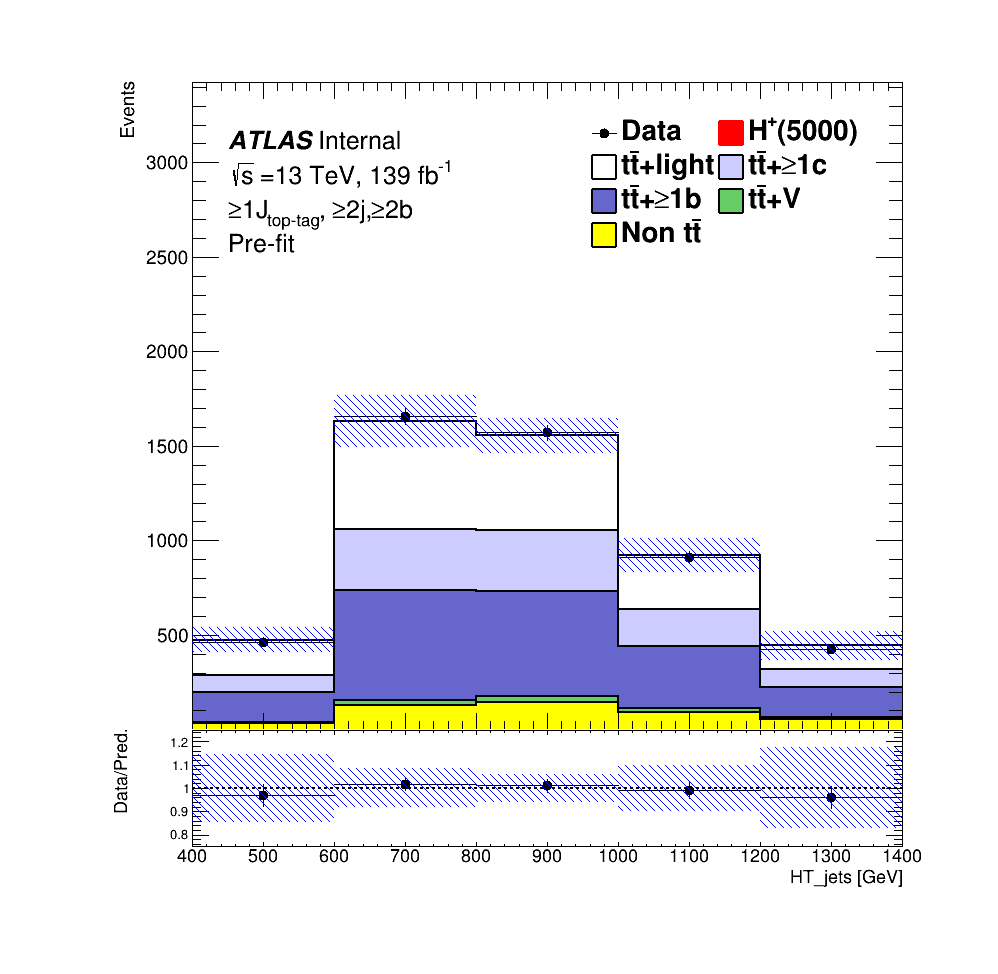
\includegraphics[width=0.45\textwidth]{images/FitTest/Prefit_Hp5000_blind_w_ttl_scaled_CR1.png}
  }
  \subfloat[]{
    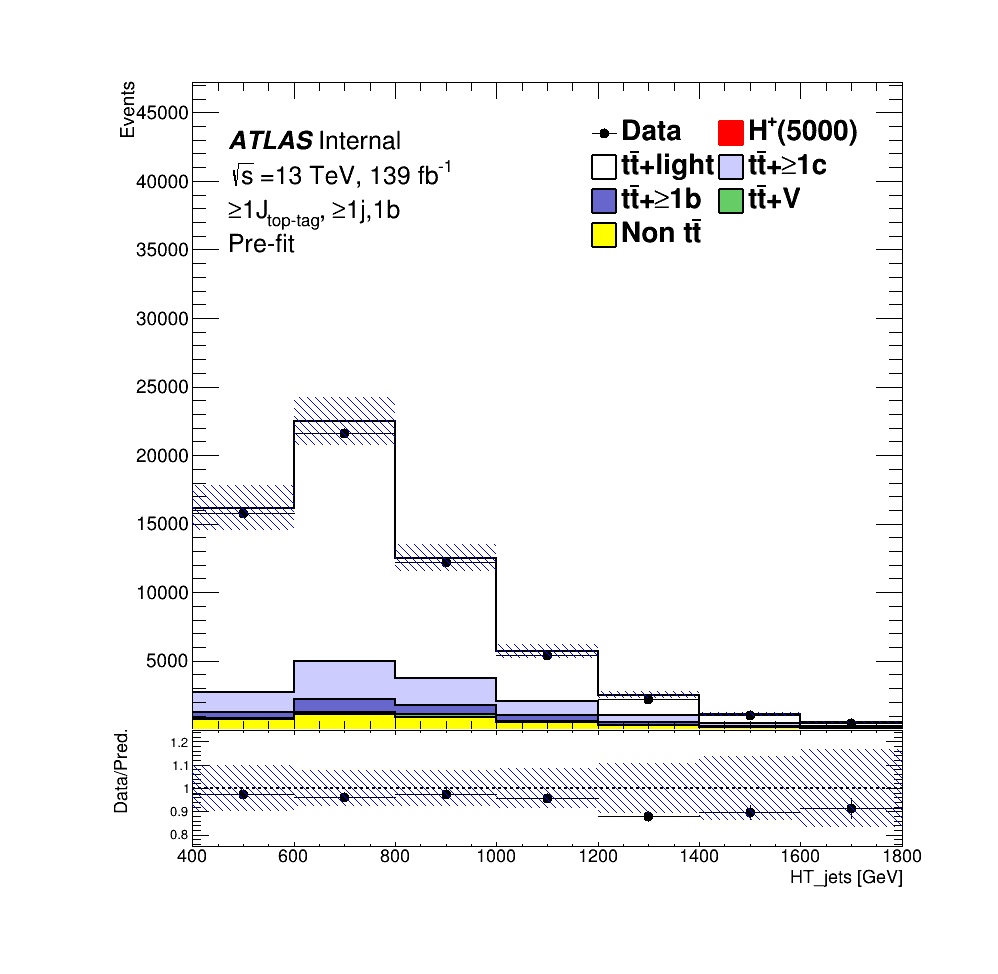
\includegraphics[width=0.45\textwidth]{images/FitTest/Prefit_Hp5000_blind_w_ttl_scaled_CR2.png}
  }
  \caption{Pre-fit plots in the CR1 (left) and CR2 (right) for 5000 GeV mass hypothesis of $H^{+}$ signal. The blinded bins aren't plotted. $t\Bar{t}+\text{light}$ MC events are scaled by 0.856. The uncertainties of $+0.074$ and $-0.070$ are included as systematics. The scale factor and uncertainties are the ratio of fiducial cross-sections of collision data and $t\Bar{t}$ MC (PP8), which are obtained by $t\Bar{t}$ cross-section measurement analysis using boosted top-quarks in $\ell+\text{jets}$ channel.}
  \label{fig:Prefit_Hp5000_Blind_with_ttlight_constrained}
\end{figure}


\subsubsection{Fit results}
Figure \ref{fig:NormFactors_Hp1000_Blind_with_ttlight_constrained} to \ref{fig:NormFactors_Hp5000_Blind_with_ttlight_constrained} show the BOnly fit result of $t\Bar{t}+\text{HF}$ normalization for each $H^{+}$ signal mass hypothesis. These results are consistent with the results with $t\Bar{t}+\text{light}$ free-floating in the fit (Section \ref{subsubsec:DataFitResults}).

\begin{figure}[H]
  \centering
  \subfloat[]{
    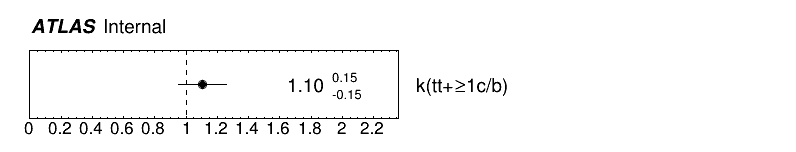
\includegraphics[height=0.20\textwidth]{images/FitTest/NormFactors_Hp1000_blind_w_ttl_scaled.png}
    \label{fig:NormFactors_Hp1000_Blind_with_ttlight_constrained}
  }\par
  \subfloat[]{
    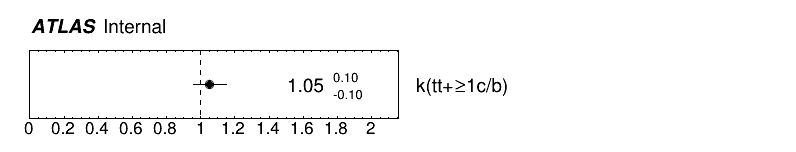
\includegraphics[height=0.20\textwidth]{images/FitTest/NormFactors_Hp2000_blind_w_ttl_scaled.png}
    \label{fig:NormFactors_Hp2000_Blind_with_ttlight_constrained}
  }\par
  \subfloat[]{
    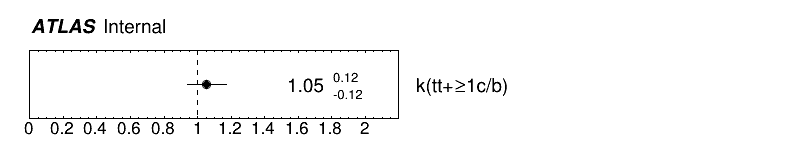
\includegraphics[height=0.20\textwidth]{images/FitTest/NormFactors_Hp3000_blind_w_ttl_scaled.png}
    \label{fig:NormFactors_Hp3000_Blind_with_ttlight_constrained}
  }\par
    \subfloat[]{
    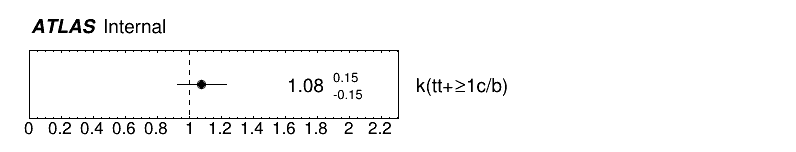
\includegraphics[height=0.20\textwidth]{images/FitTest/NormFactors_Hp4000_blind_w_ttl_scaled.png}
    \label{fig:NormFactors_Hp4000_Blind_with_ttlight_constrained}
  }\par
    \subfloat[]{
    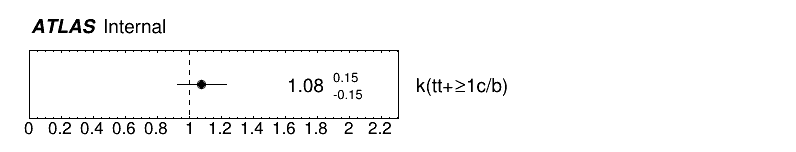
\includegraphics[height=0.20\textwidth]{images/FitTest/NormFactors_Hp5000_blind_w_ttl_scaled.png}
    \label{fig:NormFactors_Hp5000_Blind_with_ttlight_constrained} 
  }
  \caption{BOnly fit results of $t\Bar{t}+\text{HF}$ normalization for from 1000 to 5000 GeV $H^{+}$ signal mass hypotheses.}
  \label{fig:NormFactors_Blind_with_ttlight_constrained}
\end{figure}